\documentclass{ezb}
\usepackage[]{todonotes}
\usepackage{amsmath}
\usepackage{gensymb}
\usepackage{wrapfig}
\usepackage{longtable}
\usepackage{amssymb}
\usepackage[colorlinks,        	% Links ohne Umrandungen in zu wählender Farbe
   linkcolor=black,   			% Farbe interner Verweise
   filecolor=black,   			% Farbe externer Verweise
   citecolor=black    			% Farbe von Zitaten
]{hyperref}
\usepackage{booktabs}

\renewcommand{\thesubsection}{\alph{subsection}}
\begin{document}

% \maketitle{Nummer}{Abgabedatum}{Tutor-Name}{Gruppennummer}
%           {Teilnehmer 1}{Teilnehmer 2}{Teilnehmer 3}
\maketitle{05.06.15}{Udo Frese}{1}{Annika Ofenloch - 2992807 - ofenloch@uni-bremen.de}{Frank Ihle - 3010158 - fihle@uni-bremen.de}{Simon Schirrmacher - 4000884 - simons@informatik.uni-bremen.de}{Noshaba Cheema - ncheema@uni-bremen.de}

%-------Text-Start------------------------------------------
\section{Ballspiele II}

\begin{lstlisting}[language=C++, caption=Computes the perspective projection (in pixel) of \textbackslash c p]
int CameraCalibration::project (double& x, double& y, const VVector& pInWorld) const
{
	// TODO: implement (1P)
	Transform worldInCamera;
	inverse(worldInCamera, cameraInWorld);
	VVector pInCamera = worldInCamera * pInWorld;

	// avoid division by zero
	if (pInCamera[2] == 0) return 0;

	x = centerX + alpha * pInCamera[0] / pInCamera[2];
	y = centerY + alpha * pInCamera[1] / pInCamera[2];

	// check if behind camera
	if (pInCamera[2] < 0) return 0;
	// check if inside image
	return isInside(x, y) + 1;
}
\end{lstlisting}

\begin{lstlisting}[language=C++, caption=Project a sphere of \textbackslash c radius at \textbackslash c p into the image]
int CameraCalibration::project (double& x, double& y, double& r, const VVector& pInWorld, double radius) const
{
	// TODO: implement (1P)
	Transform worldInCamera;
	inverse(worldInCamera, cameraInWorld);
	VVector pInCamera = worldInCamera * pInWorld;

	// avoid division by zero
	if (pInCamera[2] == 0) return 0;

	x = centerX + alpha * pInCamera[0] / pInCamera[2];
	y = centerY + alpha * pInCamera[1] / pInCamera[2];
	r = alpha * radius / pInCamera[2];

	// check if behind camera
	if (pInCamera[2] < 0) return 0;
	// check if inside image
	return isInside(x, y) + 1;
}
\end{lstlisting}

\begin{lstlisting}[language=C++, caption=Compute the world position of an image sphere]
bool CameraCalibration::generate (VVector& pInWorld, double x, double y, double r, double radius) const
{
	// TODO: implement (1P)
	if(r <= 0) return false;

	VVector pInCamera;
	pInCamera[3] = 1;
	pInCamera[2] = alpha * radius / r;
	pInCamera[1] = (y - centerY) * pInCamera[2] / alpha;
	pInCamera[0] = (x - centerX) * pInCamera[2] / alpha;

	pInWorld = cameraInWorld * pInCamera;

	// check if input of generate is equal to output of project
	double xImage, yImage, rImage;
	project(xImage, yImage, rImage, pInWorld, radius);
	assert("project(generate(INPUT)) must be equal to INPUT!" && 
		fabs(x - xImage) + fabs(y - yImage) + fabs(r - rImage) < 0.1);
	return true;
}
\end{lstlisting}

\begin{lstlisting}[language=C++, caption=The parameters used by this algorithm]
ParticleFilter::Parameters::Parameters ()
// TODO: choose good parameter (1P)
:ballRadius(0.1), sigmaVelocity(0.5), sigmaImage(2), deltaT(1.0 / 25), waitUntilSecondObservation(3.0 / 25), nrOfParticles(200)
{
  g[0] = 0;
  g[1] = 0;  
  g[2] = -9.81;
  g[3] = 0;
}
\end{lstlisting}

\begin{lstlisting}[language=C++, caption=Integrate an observation of the ball during initialization]
void ParticleFilter::Particle::observeInit (double x, double y, double r)
{
	// TODO: implement (2P)
	double sigma = filter->param.sigmaImage;
	VVector p;
	// add noise
	x += sigma * randomGaussian();
	y += sigma * randomGaussian();
	r += sigma * randomGaussian();
	if (filter->camera.generate(p, x, y, r, filter->param.ballRadius)) {
		if (state == POSITIONDEFINED) {
			double dT = time - timeOfLastObservation;
			// determine velocity after waitUntilSecondObservation has passed
			if (dT > filter->param.waitUntilSecondObservation) {
				// acceleration added to initial velocity for analytical approach
				velocity = (p - position) / dT + filter->param.g * dT * .5;
				position = p;
				state = FULLDEFINED;
				timeOfLastObservation = time;
			}
		}
		else {
			// determine initial position of particle
			position = p;
			state = POSITIONDEFINED;
			timeOfLastObservation = time;
		}
	}
	// for a better result, particles outside of field of view can be already winthdrawn in the initialization
	else weight = 0;
	if (position[2] < 0) weight = 0;
}
\end{lstlisting}

\begin{lstlisting}[language=C++, caption=Integrate an observation of the ball once the particle is fully initialized]
void ParticleFilter::Particle::observeRegular (double x, double y, double r)
{
	// TODO: implement (1P)
	double dx, dy, dr, sigma = filter->param.sigmaImage;
	// ignore particle if behind camera
	if (!filter->camera.project(dx, dy, dr, position, filter->param.ballRadius)) 
		weight = 0;
	else {
		// weight particle
		dx = x - dx;
		dy = y - dy;
		dr = r - dr;
		weight *= exp(-(dx*dx + dy*dy + dr*dr) / (2 * sigma * sigma));
	}
	timeOfLastObservation = time;
}
\end{lstlisting}

\begin{lstlisting}[language=C++, caption= Time \textbackslash c deltaT has passed. Proceed to the next image and update the particles accordingly.]
void ParticleFilter::dynamic ()
{
	// TODO: implement (included with Particle::dynamic)
	for (int i = 0; i < particle.size(); ++i)
		particle[i].dynamic(param.deltaT);
}

void ParticleFilter::Particle::dynamic (double deltaT)
{
	// TODO: implement (2P)
	if (state == FULLDEFINED) {
		VVector n = { randomGaussian(), randomGaussian(), randomGaussian(), 0};
		// analytical approach
		position += deltaT * velocity + deltaT * deltaT * filter->param.g * .5;
		velocity += deltaT * filter->param.g + filter->param.sigmaVelocity * sqrt(deltaT) * n;
	}
	time += deltaT;
}
\end{lstlisting}

\begin{lstlisting}[language=C++, caption= A ball has been seen with image \textbackslash c x y and radius \textbackslash c r.]
void ParticleFilter::observe (double x, double y, double r)
{
	// TODO: implement (included with Particle::observe)
	for (int i = 0; i < particle.size(); ++i)
		particle[i].observe(x, y, r);
}
\end{lstlisting}

\begin{lstlisting}[language=C++, caption=Initialize the particle filter with \textbackslash c nrOfParticles particles]
void ParticleFilter::createSamples (int nrOfParticles)
{
	// TODO: implement (included with ParticleFilter::Parameters::Parameters)
	double weight = 1.0 / nrOfParticles;
	for (int i = 0; i < nrOfParticles; ++i)
		particle.push_back(Particle(this, weight));
}
\end{lstlisting}

\begin{lstlisting}[language=C++, caption=Draw particles from the particle set]
void ParticleFilter::resample (int nrOfParticles)
{
	// TODO: implement (1P)
	// 'j' and 'weightUpToJ' just for solution in lecture
	double totalWeight = 0, weightUpToJ = 0;
	int j = -1;
	vector<Particle> pNew;

	// calculate total weight
	for (int i = 0; i < particle.size(); ++i)
		totalWeight += particle[i].weight;

	double normWeight = totalWeight / nrOfParticles, unitWeight = 1.0 / nrOfParticles;
	// initial "wheel of fortune" pointer
	double weightChosen = randomUniform() * normWeight;

	for (int i = 0; i < nrOfParticles; i++) {

		// solution from lecture creates an infinite loop because the Gaussian distribution becomes 0 at some points
		// where the particle is too far from the actual cirle (numerical underflow)

		/*
			while (weightChosen >= weightUpToJ) {
				j++;
				weightUpToJ += particle[i].weight;
			}
			pNew.push_back(particle[j]);
			pNew.back().weight = unitWeight;
			weightChosen += normWeight;
		*/

		// current "wheel of fortune" pointer
		weightChosen -= particle[i].weight;
		// add normWeight to the current pointer until the wanted wight is archieved
		while (weightChosen <= 0) {
			pNew.push_back(particle[i]);
			pNew.back().weight = unitWeight;
			// next "wheel of fortune" pointer
			weightChosen += normWeight;
		}
	}
	// make sure sizes are equal
	assert("Resampled particles must have the size of nrOfParticles" && pNew.size() == nrOfParticles);
	particle = pNew;
}
\end{lstlisting}
\newpage
\section{Freistoß (4 Punkte)}
Bei einer Fußball-TV-Übertragung soll für den Zuschauer die Zone in das Bild eingezeichnet werden, auf der sich kein Gegenspieler bei einem Freistoß befinden darf.
\subsection{Allgemein}
Der Algorithmus orientiert sich an bekannten Objekten, deren Dimensionen im physikalischen Raum ihm bekannt sind. Die meisten Bemaßungen auf einem Fußballfeld sind festgeschrieben und falls es hiervon Abweichungen gibt, können diese vor Spielbeginn eingeholt und händisch eingetragen werden.\\
\linebreak
Das Fußballfeld ist rechteckig, aber je nach Blickwinkel der Kamera ergeben sich Bildverzerrungen (beispielsweise erscheint der Platz, wenn die Kamera flach, von der Seite sowie mittig auf das Spielfeld schaut, trapezförmig). Diese Verzerrung muss ebenso beim Kreis berücksichtigt werden. So wird aus dem Kreis eine Ellipse, deren kurze Diagonale umso größer wird, je näher die Ellipse an der Kamera ist. Diese Verzerrung kann durch die Kameragleichung ermittelt werden (siehe Gleichung \ref{eq:Kameragleichung})\\
\linebreak
Wenn nun bekannt ist, mit welchen Parametern die Ellipse eingezeichnet werden soll, gibt es hierfür zwei Möglichkeiten, diese um den Ball, als Mittelpunkt zu zeichnen. Zum einen kann statisch festlegen werden, dass das Kamerabild genau an einer Stelle stehen bleibt und erst beim Anspielen wieder geschwenkt werden darf, da sich ab hier der Kreis wieder auflösen soll - so muss die Zone nur einmal berechnet und eingetragen werden. Für die nachfolgenden Bilder
kann diese dann einfach rein kopiert werden. \\
\linebreak
Die andere Möglichkeit besteht darin, den Freistoß-Kreis beim Zoom-Vorgang zu zeigen. Hierfür werden mindestens zwei Bilder benötigt, auf denen Objekte zu sehen sind, deren reale Größe bekannt sind (siehe \ref{b:skaliergr} Skaliergrößen). Im Mittelpunkt der Bilder ist der Ball und es werden wie gewohnt die Ellipsen berechnet. Da sich aber beim Zoomen die Zone im Folgebild vergrößert, kann nun ein $\vartriangle r$ berechnet werden und für die nächsten Aufnahmen (vor allem für diese, wo kein Objekt mit bekannter Größe zu erkennen ist) der Radius und dadurch die Ellipse definiert werden. Da dies einer linearen Zoom-Funktion entspricht, funktioniert dieses Verfahren ausschließlich bei konstanter Vergrößerungsgeschwindigkeit. Wenn mehr als zwei Aufnahmen zur Berechnung von $\vartriangle r$ verwendet und deren Ergebnis gemittelt werden, lässt sich dieser Faktor genauer einstellen.\\
\linebreak
\textbf{UPDATE }Optional kann der Kreis farblich markiert werden, wenn ein Gegenspieler sich innerhalb des Kreises befindet. Hierfür tippt der Kameramann die Personen an, die sich innerhalb der Zone befinden dürfen. Anschließend wird deren Positionen immer mit dem vorhergehenden Bild verglichen, um eine Falschmeldung auszuschließen, wenn die Signalfarbe gesetzt werden soll. Gegenspieler im Kreis werden über deren Position und farbliche Unterschiede zum jeweiligen Boden erkannt.\\
\linebreak
\textbf{UPDATE }Um Verwechslungen und Fehlausstrahlung zu vermeiden soll der Kameramann zum einen, einen Bereich um den Kreis angeben, mit welcher der Algorithmus über Hough zur Ballposition kommt. Zum anderen soll der auszustrahlende Kreis nochmal von einer Person bestätigt werden, ob dieser ungefähr in Position und Größe richtig ermittelt wurde.
\subsection{Skalierobjekte}\label{b:skaliergr}
Nachfolgend, Beispiele für Objekte mit bekannten Ausmaßen, mit deren Hilfe letztlich die Freistoßzone definiert werden kann: Torlatte und -pfosten, Rasenmuster sowie die weiße Linien (darunter: Seiten- und Mittellinien, Strafraum und Anstoßkreis).\\
\linebreak
\textbf{UPDATE }Damit der Algorithmus weiß, um welches Skalierobjekt es sich gerade handelt soll entweder der Kameramann angeben, dass im Blickpunkt sich z.B.: das Tor befindet. Oder es muss noch ein automatischer Klassifizierungsalgorithmus hinzugefügt werden, welcher z.B.: den Mittelkreis über dessen Form, oder den Strafraum über seine rechteckige Form vor dem Tor erkennt.
\subsection{Kameraeinstellung}
Ein Bildpunkt im Weltkoordinatensystem kann auf das Kamerasystem mit nachfolgender Gleichung umgerechnet werden:\\
\begin{small}
\begin{equation}
\left(
\begin{array}{c}
      u \\
      v
\end{array}
\right)
=
\left(
\begin{array}{c}
      u_{0} \\
      v_{0}
\end{array}   
\right)
+ \alpha \cdot d_{\kappa1 ,\kappa2}(p(T^{-1}_{W\leftarrow C}\cdot p^{W})) 
\label{eq:Kameragleichung}
\end{equation}
\end{small}
Die Transformationsmatrix beinhaltet nur die Verschiebung des Balls zum Ursprung und die Rotation um die Z- und X- Achse, die die Perspektive, Schwenken und das Nicken ausgleichen können. Da die Kamera aber nicht gieren kann, wäre eine Rotation um die Y-Achse nur nötig, um eine Kamerafehleinstellung auszugleichen (?).\\
\linebreak
Hier soll nun $\alpha_{r}$ die Verdrehung um die Z-Achse veranschaulichen. $\alpha_{r}$ ist der Winkel zwischen dem ursprünglichen und dem, um eine Achse verdrehtes Koordinatenkreuz. Dieser ist variabel und nähert sich immer mehr $\frac{\pi}{2}$, je mehr er sich der Kamera bzw. der blauen Linie nähert. Repräsentativ für den anderen Winkel soll die Winkelberechnung anhand der Beziehung für $\alpha_{r}$ erläutert werden, die in Abb. \ref{abb:alpharBerechnung} veranschaulicht ist.\\
\linebreak
Die blaue Strecke teilt das Feld in zwei Bereiche auf, sie ist gleichzeitig die Spiegelachse für $\alpha_{r}$ und orientiert sich an der Kameraposition (hier ist $x=0$). So haben Strecken, die parallel zur Torlinie verlaufen, aus dieser Perspektive in der linken Hälfte eine positive Steigung und in der rechten eine negative Steigung. Aus diesem Grund muss hier auch eine Fallunterscheidung gemacht werden, sodass $\alpha_{r}$ immer über das Winkel/Positionsverhältnis berechnet wird, wie in Gleichung \ref{eq:alphar} beschrieben. Eine Ähnliche Berechnung muss für den Verkippungswinkel (um X) des Koordinatenkreuzes durchgeführt werden. [Hängt $\beta$ von der Blauen linie ab, oder ist beta überall gleich? Wenn überall gleich bitte nachfolgenden satz streichen/umschreiben]. $\beta$ wird dann ähnlich wie $\alpha$ über das Verhältnis von min. und max. Ballposition in Z Richtung ermittelt\\
\begin{equation}
\alpha_{r} = 
\begin{cases}
	[\frac{\pi}{2} - (\frac{\pi}{2}-\alpha_{1,min})]\frac{b'}{x} & wenn \ x\geq 0  \\
    [\frac{\pi}{2} - (\frac{\pi}{2}-\alpha_{2,min})]\frac{b-b'}{x} & wenn \ x\leq 0 \\
\end{cases}
\label{eq:alphar}
\end{equation}
\begin{figure}[!h]
\centering
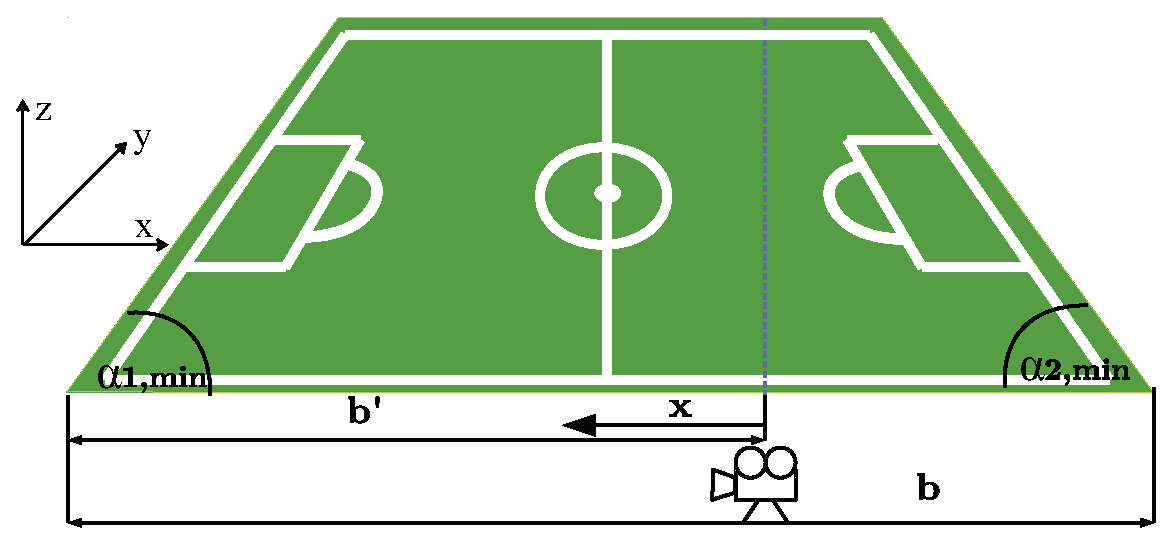
\includegraphics[scale=0.6]{./ar.eps}
\caption{Veranschaulichung für die $\alpha_{r}$-Berechnung}
\label{abb:alpharBerechnung}
\end{figure}
\subsection{Beurteilung}
Da beim Fußball schon wenige cm entscheidend sind, sollte der einzusetzende Algorithmus genaue Ergebnisse liefern, da \glqq Fehlentscheidungen\grqq \ ansonsten den Zuschauer verärgern können. Die unter diesen Bedingungen, gezeigten Methoden haben vermutlich nur eine begrenzte Genauigkeit, je nachdem wie exakt ein Objekt mit bekannter Größe erfasst wird (Negativbeispiel: Auflösung des Fußballs bei Aufnahme aus der Entfernung).
\section{Der einäugige Ballfangkönig (1 Punkt)}
Um den Skalenmaßstab aus den Messungen zu bestimmen, soll eine Analyse der Situation durchgeführt werden. Zum einen lässt sich der Skalenmaßstab über die Tiefenschärfe und zum anderen über die Flugbahn des Balls ermitteln. Bei der Flugbahn werden zwei Ansätze betrachtet. Im Folgenden werden die drei Verfahren kurz erläutert.
% Tiefenschärfe-Verfahren (Kamera-Parameter)
\subsection{Verfahren mit Hilfe der Tiefenschärfe}
Die Brennweite bestimmt den Abstand Linsenhauptebene und ihrem Brennpunkt. Ist nun also diese Brennweite (Abstand in z.B.: Metern) bei einer Kamera gegeben, so kennt man den Abstand eines Objekts zur Linse, wenn dieses den höchsten Schärfegrad erreicht hat. Dies kann beispielhaft bei unserem Ballwurfszenario implementiert werden. Hier wird einfach für jedes Bild die Kantenbreite über Sobel berechnet und das Bild, mit der der Ball die größten Sobellänge erreicht, ist dann dem Fokus der Kameralinse am nächsten. Die Genauigkeit der Methode hängt zum einen von der Genauigkeit der Brennweitenangabe und zum anderen von der Möglichkeit, den Ball genau im Brennpunkt erfassen zu können, ab.\\
\linebreak
Der Balldurchmesser kann demnach mit Hilfe der internen Kamerabemaßungen und dem Strahlensatz ermitteln werden. Wenn $\overline{AB}$ die Breite des Fotochips, $\overline{A'B'}$ die Breite des sich auf der Linse befindenden Bilds, $\overline{A''B''}$ der Balldurchmesser, $d_{1}$ der Abstand vom Fotochip zur Linsenhauptebene und $d_{2}$ die Brennweite ist, kann $\overline{A''B''}$  wie folgt berechnet werden (siehe. Abb \ref{abb:Strahlensatz}):\\
\linebreak
\begin{figure}[!h]
\centering
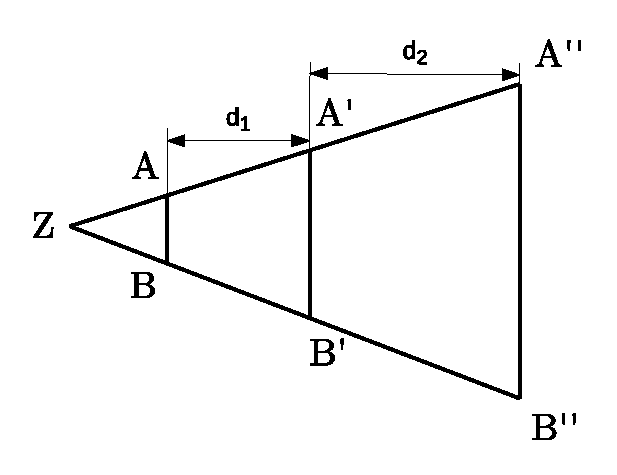
\includegraphics[scale=0.6]{./Strahlensatz.eps}
\caption{Veranschaulichung für die Balldurchmesserberechnung mit Hilfe der Tiefenschärfe.}
\label{abb:Strahlensatz}
\end{figure}
\begin{center}
$\frac{\overline{AB}}{\overline{A'B'}} = \frac{\overline{ZA}}{\overline{ZA'}} = \frac{\overline{ZA}}{\overline{ZA}+\overline{AA'}}$\\ \vspace{0.5cm}
$(\overline{ZA}+\overline{AA'})\frac{\overline{AB}}{\overline{A'B'}}-\overline{ZA}=0$\\ \vspace{0.5cm}
$\overline{ZA}=\frac{\overline{AA'}\frac{AB}{A'B'}}{1-\frac{AB}{A'B'}}$
\end{center}
mit
\begin{center}
$\overline{A'A} = \sqrt{d_{1}^{2}+(\frac{\overline{A'B'}}{2}-\frac{\overline{AB}}{{2}})^{2}}$\\
\end{center}
dann erhält man über
\begin{center}
$\frac{\overline{AB}}{\overline{A''B''}} = \frac{\overline{ZA}}{\overline{ZA''}} = \frac{\overline{ZA}}{\overline{ZA}+\overline{AA'}+\overline{A'A''}} $\\
\end{center}
mit
\begin{center}
$\overline{A'A''} = \sqrt{d_{2}^{2}+(\frac{\overline{A''B''}}{2}-\frac{\overline{A'B'}}{{2}})^{2}}$\\
\end{center}
das gesuchte $\overline{A''B''}$ mit folgender Berechnung:\\
\begin{center}
$\overline{A''B''} = \frac{\overline{ZA}+\overline{AA'}+\overline{A'A''}}{\overline{ZA}}\overline{AB}$
\end{center}
\subsection{Verfahren mit Hilfe der Ballflugbahn}
% Bahngleichung
\subsubsection*{Erster Ansatz}
Des Weiteren lässt sich der Skalenmaßstab über die Flugbahn des Balls berechnen, welche aus den vorhandenen Messungen hervorgeht. Es handelt sich hierbei um einen schrägen Wurf.
Die Aufnahmezeit der einzelnen Frames ist bekannt, sodass über den Wurfwinkel $\alpha$ die Anfangsgeschwindigkeit $v_0$ ermittelt werden kann, wenn angenommen wird, dass die Ballposition auf dem ersten Frame den Start repräsentiert. $v_0$ setzt sich aus den Komponenten $v_x$ und $v_y$ zusammen und ist Abhängigkeit vom Abwurfwinkel $\alpha$ (siehe Abbildung \ref{abb:geschwindigkeiten}). $v_y$ stellt hierbei die Geschwindigkeit in y-Richtung und $v_x$ die Geschwindigkeit in x-Richtung dar und lassen sich über die folgenden Gleichungen ausdrücken:
\begin{center}
$v_x = v_0 * cos(\alpha)$ \\
$v_y = v_0 * sin(\alpha)$
\end{center}
\begin{figure}[!h]
	\centering
	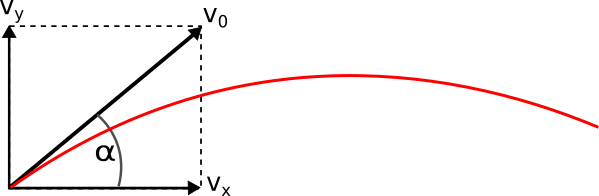
\includegraphics[scale=0.8]{./img/geschwindigkeitsrichtung.png}
	\caption{Geschwindigkeitsvektoren $v_0$, $v_x$ sowie $v_y$}
	\label{abb:geschwindigkeiten}
\end{figure}
Mittels des Geschwindigkeit-Zeit-Gesetzes, wo ebenso die Erdbeschleunigung ($g \approx 9.81m/s^2$) und Steigzeit $t_H$ einbezogen wird, lässt sich die Geschwindigkeit $v_y$ bei einem schrägen Wurf wie folgt berechnen:
\begin{center}
$v_y = v_0 * sin(\alpha) - g * t_H$
\end{center}
Da $v_y$ am höchsten Punkt der Bahnkurve gleich 0 ist, lässt sich die Gleichung nach $v_0$ umstellen. Bei $t_H$ handelt es sich um die vergangene Zeit vom ersten Bild (Start bei $t_1$) bis zum Bild mit dem höchsten Punkt der Bahnkurve (Maximum bei $t_2$), wie in Abbildung \ref{abb:ballflugbahn} zu sehen ist. Da alle Parameter bekannt sind, kann die Anfangsgeschwindigkeit $v_0$  mit der Gleichung 
\begin{center}
	$v_0 = \dfrac{g * t_H}{sin(\alpha)}$
\end{center}
berechnet werden.
\begin{figure}[!h]
	\centering
	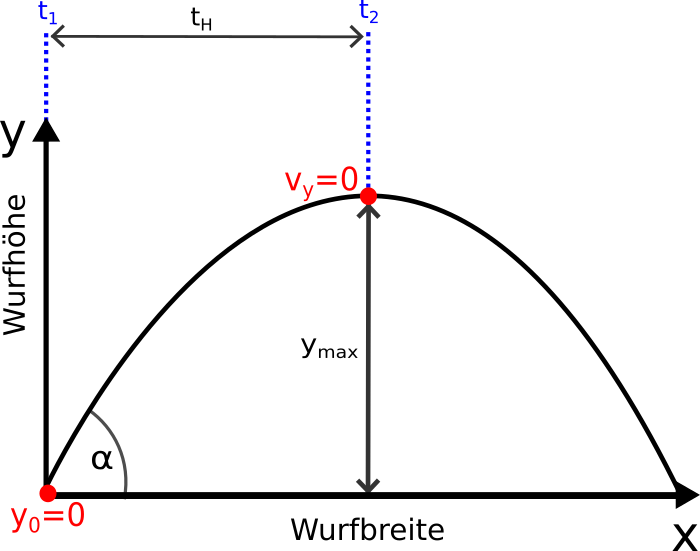
\includegraphics[scale=1.5]{./img/BallflugbahnAnsatz1.png}
	\caption{Ballflugbahn}
	\label{abb:ballflugbahn}
\end{figure}
Anschließend kann die maximale Wurfhöhe $y_{max}$ unter Verwendung des Ort-Zeit-Gesetz über die nachfolgende Gleichung ermittelt werden, wobei $y_0$ gleich 0 ist:
\begin{center}
$y_{max} = y_0 + v_0 * sin(\alpha) * t_H - g * (t_{H})^{2}$
\end{center}
Wenn nun die Länge der maximalen Wurfhöhe, wie in Abbildung \ref{abb:ballflugbahn} zu sehen ist, bekannt ist, verfügt man über einen Skalenmaßstab mit dem zum Beispiel der Balldurchmesser bestimmt werden kann. Es handelt sich hierbei jedoch nur um eine Approximation, da die z-Richtung des Wurfes nicht mit einbezogen wurde. 

Für ein genaueres Ergebnis könnte die Tiefeninformation über den zuvor beschriebenen Tiefenschärfe-Ansatz einbezogen werden, sodass beide Verfahren kombiniert werden.

\subsubsection*{Zweiter Ansatz}
Das zweite Verfahren zur Bestimmung des Skalenmaßstabs über die Ballflugbahn macht sich das Unabhängigkeitsgesetz zu nutze. Der Ball bewegt sich von der maximalen Wurfhöhe zum Zeitpunkt $t_2$ aus kurvenförmig zum Boden hin. Wenn ein weiterer Ball von der maximalen Höhe zum Zeitpunkt $t_2$ im freien Fall nach unten fallen würde, würden beide Bälle den Boden zum selben Zeitpunkt erreichen. Dieses Phänomen machen wir uns zu nutze, indem wir die Strecke $h$ für den freien Fall ermitteln, also die Entfernung von der maximalen Wurfhöhe bis zum Aufprall (siehe Abbildung \ref{abb:freierfall}). Diese Strecke $h$ wird mittels folgender Gleichung berechnet:
\begin{center}
$h = \dfrac{g * (t_H)^2}{2}$
\end{center}
\begin{figure}[!h]
	\centering
	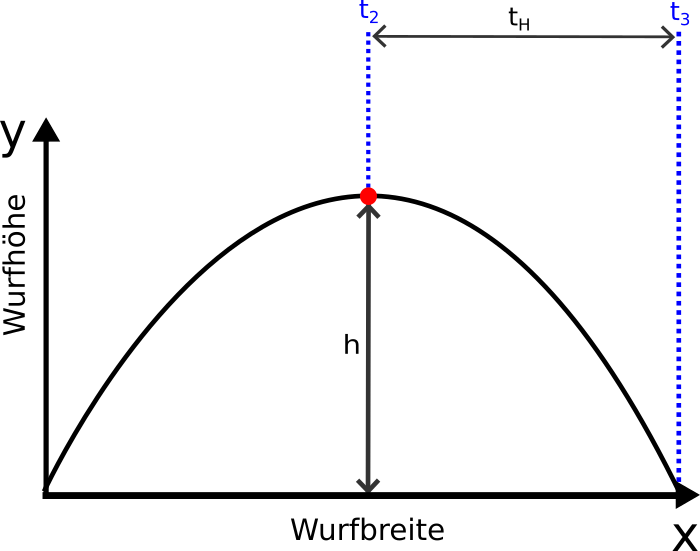
\includegraphics[scale=1.5]{./img/BallflugbahnAnsatz2.png}
	\caption{Ballflugbahn}
	\label{abb:freierfall}
\end{figure}
$t_H$ ist in diesem Fall die Fallzeit von $t_2$ bis zum Aufprall auf dem Boden. Aufgrund des Unabhängigkeitsgesetzes ist die Fallzeit über die Bildaufnahmen bekannt.
Diese Strecke $h$ stellt ebenso einen Skalenmaßstab im Bild dar, wodurch unter anderem der Balldurchmesser ermittelt werden kann. Auch bei diesem Verfahren handelt es sich nur um eine Approximation, da die z-Richtung des Wurfes nicht mit einbezogen wird.

Hinzu kommt, dass bei den Berechnungen angenommen wurde, dass kein Luftwiderstand vorhanden ist (Annahme erfolgte ebenso bei der Programmieraufgabe).




%-------Text-End------------------------------------------
\end{document}

